\documentclass[slidetop,11pt]{beamer}
%
% le texte en classe article
% \documentclass[class=article,11pt,a4paper]{beamer}
% \usepackage{beamerbasearticle}

\usepackage[T1]{fontenc} 
\usepackage[latin1]{inputenc}
\usepackage[frenchb]{babel}
\usepackage{beamerthemeshadow}
\usepackage{verbatim}
\usepackage{graphicx}
% des fontes cmsuper ou lmodern
\usepackage{lmodern}
%\usepackage{aeguill}

% Pour afficher le pdf en plein ecran
%\hypersetup{pdfpagemode=FullScreen}

% ------------------------------------------------
%-----------   styles pour beamer   --------------
% ------------------------------------------------
%
% ------------- Choix des couleurs ---------------
%\xdefinecolor{fondtitre}{rgb}{0.20,0.43,0.09}  % vert fonce
\definecolor{fondtitre}{HTML}{336E17}

%\xdefinecolor{coultitre}{rgb}{0.41,0.05,0.05}  % marron


%\definecolor{coultitre}{RGB}{10,13,13}
%\xdefinecolor{fondtexte}{rgb}{1,0.95,0.86}     % ivoire


%\xdefinecolor{fondtexte}{rgb}{1,1,1}     % blanc

%\colorlet{coultexte}{black} 

% -------------- Fioritures de style -------------
% Fait afficher l'ensemble du frame 

\beamertemplatetransparentcovered

% Supprimer les icones de navigation (pour les transparents)
\setbeamertemplate{navigation symbols}{}	
\addtobeamertemplate{footline}{\hfill\insertframenumber/\inserttotalframenumber\hspace{2em}\null}
% Mettre les icones de navigation en mode vertical (pour projection)
%\setbeamertemplate{navigation symbols}[vertical]

% ------------ Choix des th�mes ------------------

%\usecolortheme{crane}

%\useoutertheme{default}
%\useinnertheme{default}
%\useinnertheme[shadow=true]{rounded}

\beamerboxesdeclarecolorscheme{clair}{fondtitre!70}{coultitre!20}
\beamerboxesdeclarecolorscheme{compar}{coultitre!70}{fondtitre!20}





%------------ fin style beamer -------------------

% Faire apparatre un sommaire avant chaque section
% \AtBeginSection[]{
%   \begin{frame}
%   \frametitle{Plan}
%   \medskip
%   %%% affiche en d�but de chaque section, les noms de sections et
%   %%% noms de sous-sections de la section en cours.
%   \small \tableofcontents[currentsection, hideothersubsections]
%   \end{frame} 
% }
% ----------- Contenu de la page de titre --------
\subtitle{\textsc{Illustration avec FitNesse}}
\institute{CARAValence}
\date{\oldstylenums{Septembre 2012}}


% ------------------------------------------------
% -------------   D�but document   ---------------
% ------------------------------------------------
\begin{document}
%--------- �criture de la page de titre ----------
% avec la commande frame simplifi�e


\begin{frame}
\vfill
\frametitle{}
\title{Test d'acceptance}
\maketitle
\vfill


\end{frame}
%
\part{CaraValence} 
{
\begin{frame}{Sommaire}
  \small \tableofcontents[hideallsubsections]
\end{frame} 
%------------Introduction

\begin{frame}{Introduction}
\begin{block}{\only<1-1>{Qu'est ce que des tests d'acceptance ?} \only<2->{D�finition}}
\only<2->{
\begin{itemize}
		\item Un test d'acceptance est un test consommateur visant � valider l'acceptabilit� d'un produit par les consommateurs.
	\end{itemize}

}
\end{block}


	


\end{frame}

%------------------ Sommaire ---------------

%
%***************************************
%******     I           *******
%***************************************




\section[Test d'acceptance]{Test d'acceptance}
\subsection{Diff�rence entre tests unitaire et tests d'acceptances}
\begin{frame}{Test unitaire VS test d'acceptance}
\framesubtitle{Diff�rence}
\begin{block}{\only<1-1>{Pourquoi des tests d'acceptance ?} \only<2->{Pourquoi des tests d'acceptance ?}}
	\only<2->{
	\begin{itemize}
		\item xUnit: Building the Code Right   (garantit le Comment)
	  \item FitNesse: Building the Right Code (garantit le Quoi)
	\end{itemize}
}
	\end{block}
	
	\only<3->{
	\begin{alertblock}{Garantir que le code d�livr� r�pond � un besoin exprim� }
    	\begin{itemize}
				\item => Produit de la valeur
			\end{itemize}
	\end{alertblock}
	}
\end{frame}

\subsection{Sch�ma}
% avec l'environnement frame
\begin{frame}
  \frametitle{Test unitaire VS test d'acceptance}
  \framesubtitle{Sch�ma}
	\begin{figure}
			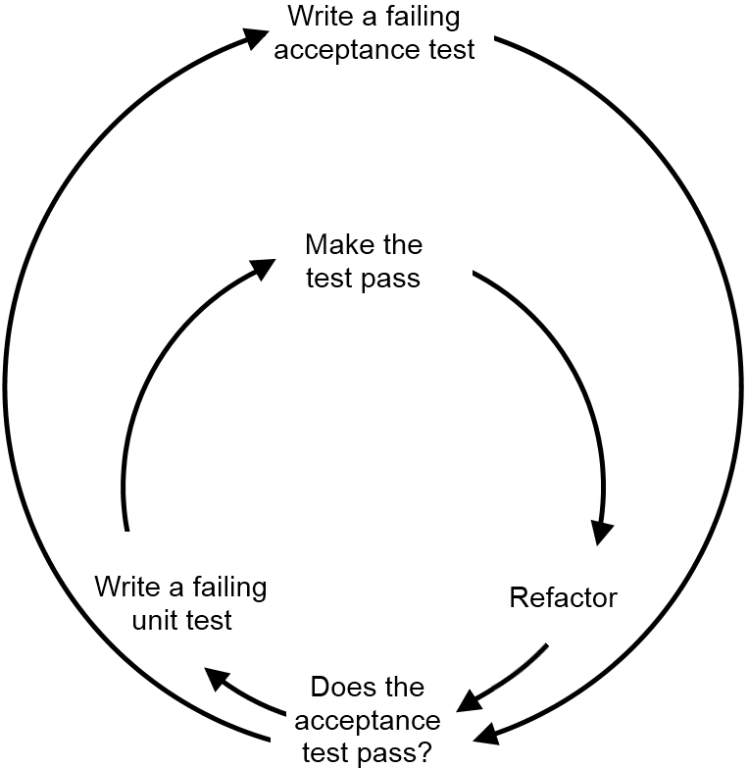
\includegraphics[width=5cm]{images/TDD-Process1.png}
			\caption{Processus test unitaire et test d'acceptance (TDD)} 
  \end{figure}	
\end{frame}


\section[L'automatisation]{Automatisation}
\subsection{Son utilit�}
\begin{frame}
  \frametitle{L'automatisation}
\framesubtitle{Son utilit�}
  \begin{block}{Les apports}
		\begin{itemize}
		\item Permettre une fr�quence de test tr�s �lev�e (int�gration continue),
	  \item Garantir un haut niveau de r�p�tabilit�,
	  \item Apporter un "formalisme" dans la description des comportements attendus.
	\end{itemize}
	\end{block}

\end{frame}

\subsection{Automatisation}
\begin{frame}
  \frametitle{Automatisation}
\begin{block}{ }
		\begin{itemize}
		\item Automatisation = Ex�cution automatique des tests (dans le cadre d'un processus d'integration continue)
	\end{itemize}
	\end{block}
NB: On pourrait aussi parler de l'automatisation de la g�n�ration des tests ;-) 
\end{frame}


\section[FitNesse]{FitNesse}
\subsection{Principe}
\begin{frame}
  \frametitle{FitNesse}
\framesubtitle{Pr�sentation}
  \begin{figure}
			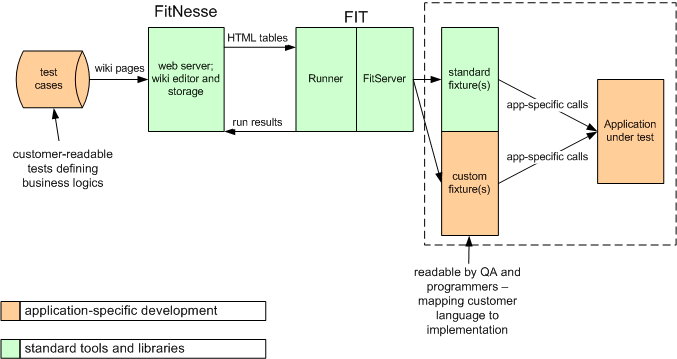
\includegraphics[width=10cm]{images/fitnese-architecture.png}
			\caption{L'architecture de FitNesse} 
  \end{figure}

\end{frame}




\subsection{Mise en oeuvre}
\begin{frame}
  \frametitle{D�monstration : Gestion d'une biblioth�que}
\framesubtitle{Diagramme de classe}
\title{titre}
 \begin{figure}
			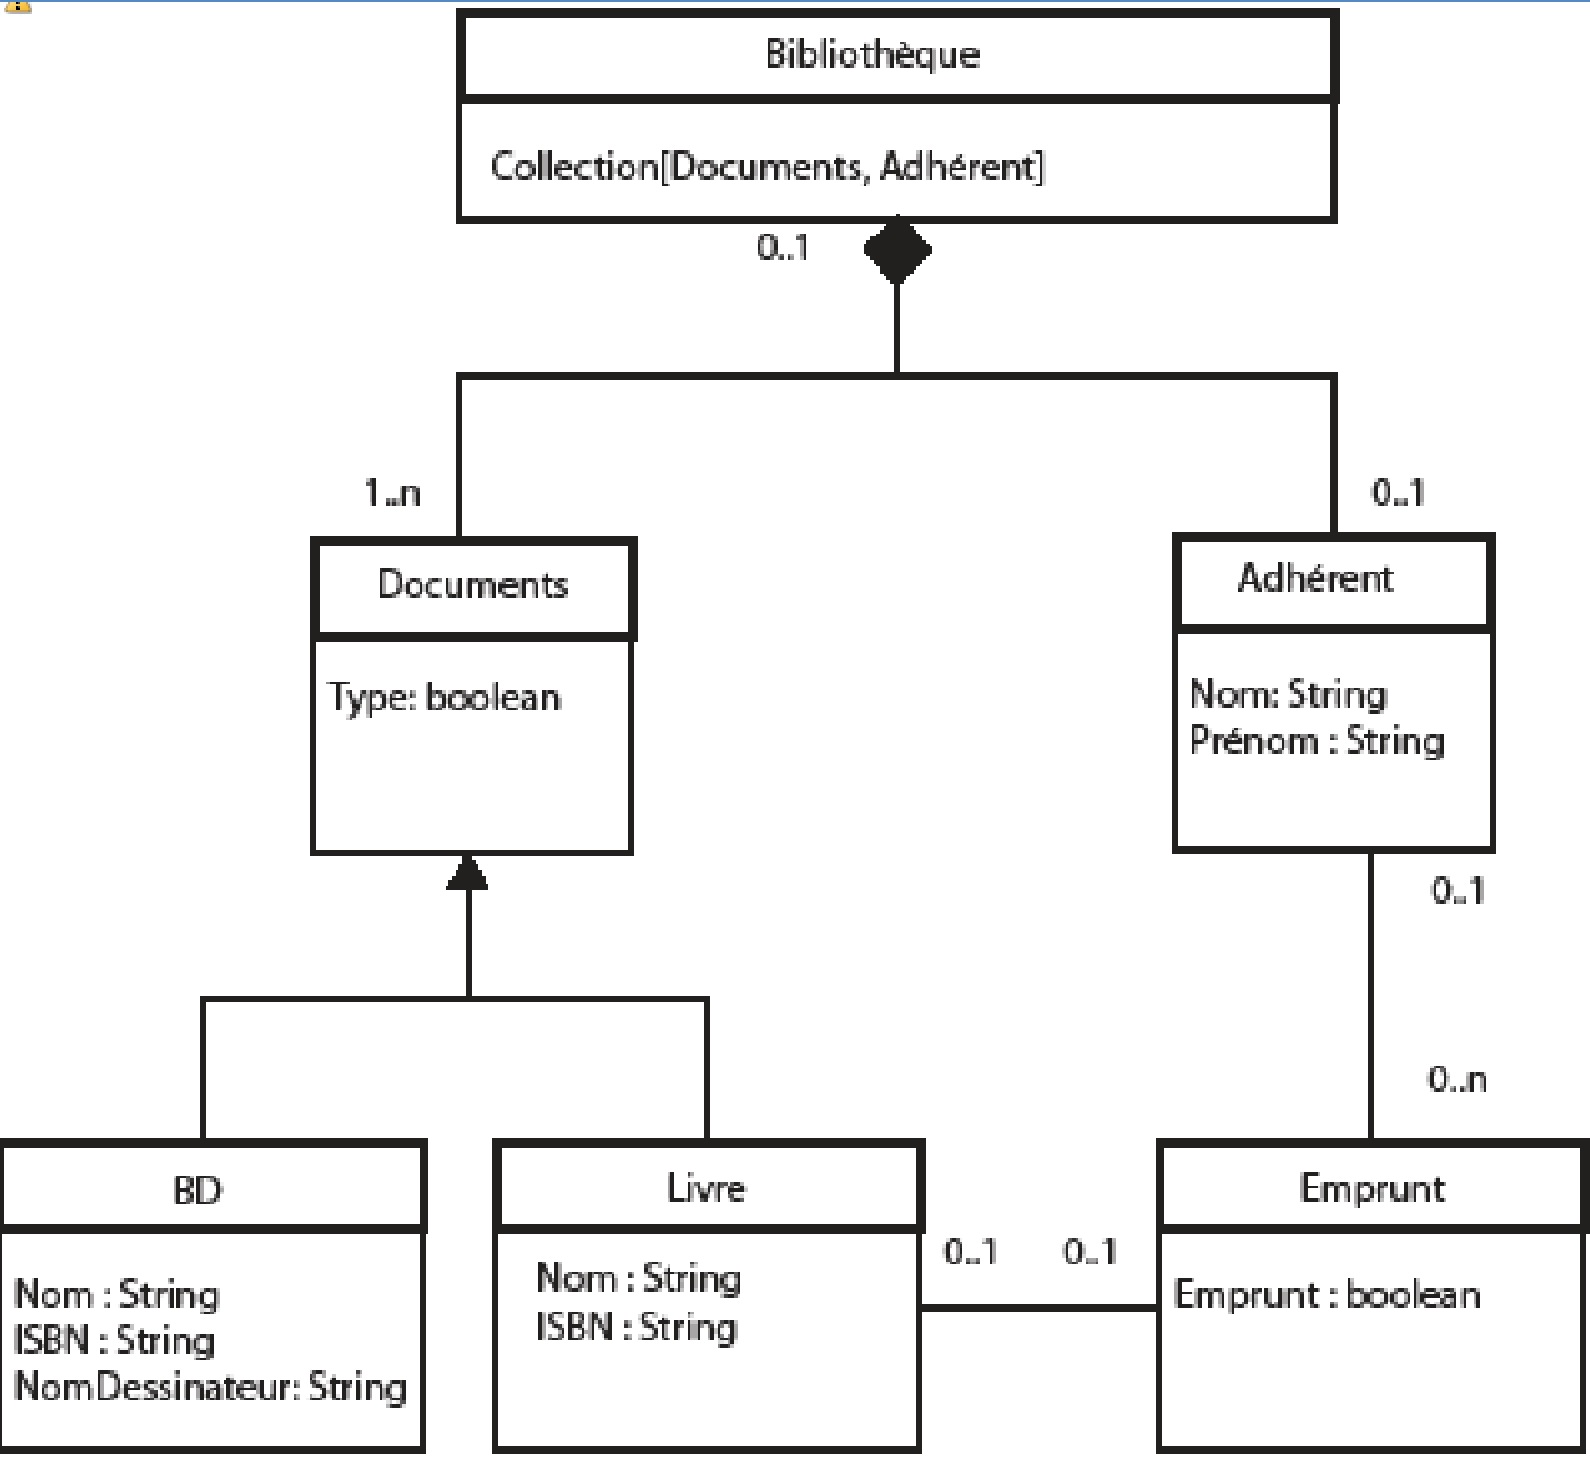
\includegraphics[width=6cm]{images/diagrammeDeClasse.jpg}
			\caption{Diagramme de classe} 
  \end{figure}
\end{frame}

\section{}
\subsection{}

\subsection{D�monstration}
\begin{frame}
  \frametitle{L'automatisation}
\framesubtitle{D�monstration : cas Markem Imaje}
  \begin{block}{D�monstration (vid�o)}
	\begin{itemize}
		\item Automatisation d'une imprimante
	\end{itemize}	
	\end{block}

\end{frame}
\section{}
\subsection{}
\begin{frame}
  \frametitle{Annexe}
\begin{block}{ }
		\begin{description}
		\item[Le test : ] Le test est l'ex�cution ou l'�valuation d'un syst�me ou d'un composant par des moyens automatiques ou manuels, pour v�rifier qu'il r�pond � ses sp�cifications ou identifier les diff�rences entre les r�sultats attendus et les r�sultats obtenus \newline
\flushright\tiny\textit{source : IEEE (Standard Glossaryof Software Engineering Terminology)}
	\end{description}
	\end{block}
 

\end{frame}
\end{document}
